% \newcommand{\prototitle}{Versuch 2 - Statistik}
% \newcommand{\Fachbereich}{Praktikum Messtechnik}
% \input{../packages/tu_header}

\newcommand{\institut}{Institut f\"ur Telekommunikationssysteme}
\newcommand{\fachgebiet}{Nachrichten\"ubertragung}
\newcommand{\veranstaltung}{Praktikum Nachrichten\"ubertragung}
\newcommand{\pdfautor}{\"Ozg\"u Dogan (326 048), Boris Henckell (325 779)}
\newcommand{\autor}{\"Ozg\"u Dogan (326 048)\\ Boris Henckell (325 779)}
\newcommand{\gruppe}{Gruppe: }
%\newcommand{\betreuer}{Betreuer: Mahmoud Felk}


\newcommand{\pdftitle}{Nachrichten\"ubertragung\ Praktikum\ 03}
\newcommand{\prototitle}{Praktikum 03 \\ Einf\"uhrung in MATLAB}


\input{../../packages/tu_header_8}


% \lstlistoflistings
\definecolor{darkgray}{rgb}{0.95,0.95,0.95}
\definecolor{darkolivegreen}{HTML}{01a801}
\definecolor{functionsBlue}{HTML}{32b9b9}
\definecolor{variableRed}{rgb}{1,0,0}
\definecolor{stringBrown}{HTML}{bc8e8e} % f geht nicht

\lstset{
        %\lstset{extendedchars=true} % Umlaute an der richtigen stelle und nicht am Anfang ausgeben
        %basicstyle=\footnotesize\ttfamily,
        basicstyle=\small,
        %
        inputencoding=utf8,
        %
        tabsize=4,
        showspaces=false,
        showtabs=false,
        showstringspaces=true, % no special string spaces
        %
        backgroundcolor=\color{darkgray}, % background
        stringstyle=\color{stringBrown}\fseries, % Strings
        keywordstyle=\color{functionsBlue}\bfseries, % keywords Blau
        identifierstyle=\color{variableRed}, % variablen
        commentstyle=\color{darkolivegreen}, %  comments
        %
        breaklines=true,
        %
        numbers=left,
        numberstyle=\tiny,
        stepnumber=1,
        numbersep=7pt,
        %
        frame=single,
        columns=flexible,
        %
        xleftmargin=-2cm,
        xrightmargin=-1.5cm,
        %
        language=Matlab
}

%---------------------------------------------------------------------
%---------------------------------------------------------------------
%---------------------------------------------------------------------

\section{Einleitung}
\begin{quote}
	In diesem Termin wurde durch praktisches Aufbauen und Testen von modulierenden
	Übertragungsstrecken das Prinzip der Amplitudenmodulation (AM) und der
	Frequenzmodulation (FM) nachvollzogen. Dafür wurde zuerst immer das nötige
	Signal erzeugt, welches dann moduliert und auch demoduliert wurde.
\end{quote}
%--------------------------------------------------------------------
%--------------------------------------------------------------------    
\section{Theorie Modulation}
\begin{quote}
        Um Signale an spezielle Kanaleigenschaften anzupassen lassen sich diese Signale durch eine Modulation in
        Amplitude und Frequenz verändern.\\
        Dies hat beispielsweise den Vorteil, dass sich die Signale anschließend mit einer Frequenz
        übertragen lassen auf der die Rauscheinflüsse geringer sind. Des weiteren entsteht durch Modulation die
        Möglichkeit mittels Multiplexing mehrere Signale gleichzeitig über einen Kanal zu übertragen und diese im
        nachhinein eindeutig unterscheinden zu können.\\
        Um das Ursprungssignal auf der Empfängerseite nutzen zu können muss es realisierbare Demodulationsmethoden
        geben.
\end{quote}


%--------------------------------------------------------------------
%--------------------------------------------------------------------    

\section{Amplitudenmodulation}
\begin{quote}
	\subsection{Theorie}
    \begin{quote}
        Bei der Amplituden Modulation wird aus dem Nutzsignal$u(t)$ mit einer variablen Amplitude und Frequenz ein
        Moduliertes Signal mit einer festen Frequenz und variabler Amplitude. Dazu wird $u(t)$ mit einem
        höherfrequenten Trägersignal $c(t)$ multipliziert. Daraus resultiert ein Signal mit der Frequenz des
        Trägersignals und einer Amplitude, die von dem Nutzsignal gesteuert wird.
        
        \begin{equation*}
        	\begin{split}
        		u_m(t) = A_c [u(t)] \cdot cos(\omega_c t)
        	\end{split}
        \end{equation*}
        
        Es gibt zwei verschiedene Möglichkeiten dieser Modulation. Erstens die Amplituden Modulation ohne Träger und die
        Amplituden Modulation mit Träger.
        
        \subsubsection{Amplitudenmodulation ohne Träger}
		\begin{quote}
			Bei dieser Art der Amplitudenmodulation wird die Amplitude linear durch das Nutzsignal gesteuert. Das bedeutet für
			die Amplitude des modulierten Signals:
			
			\begin{equation*}
            	\begin{split}
            		A_c [u(t)] = k \cdot u(t)
            	\end{split}
            \end{equation*}
            
            Welche Auswirkung diese Art der Modulation auf ein Signal hat zeigt das folgende Bild sehr anschaulich. 
            
            \begin{figure}[H]
            \centering
                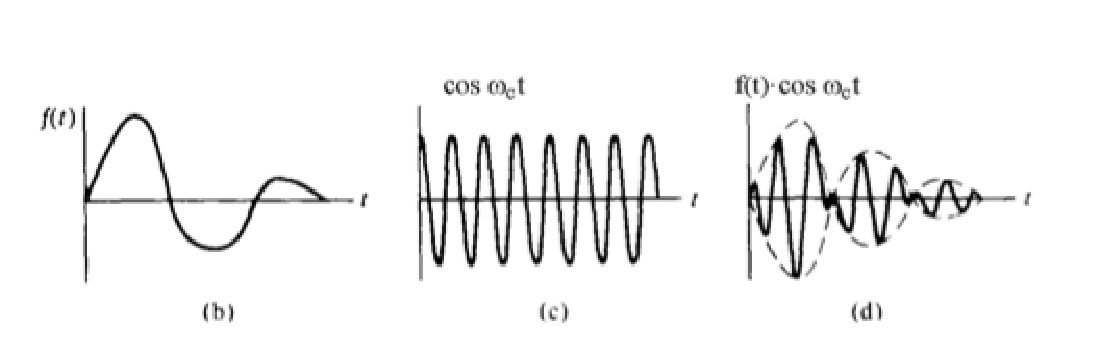
\includegraphics[scale=0.7, trim = 0cm 0cm 0cm 0cm, clip]{./Bilder/AMohneTraeger}
                    \caption{Amplitudenmodulation ohne träger}
                    \label{fig:AMohneTraeger}
                    \cite{AMohnetraeger}
            \end{figure}
    
            
            
		\end{quote}
		
		\subsubsection{Amplitudenmodulation mit Träger}
		\begin{quote}
			
		\end{quote}
        
        
    \end{quote}
    
    \subsection{Vorbereitungsaufgabe}
    \begin{quote}
        Als Vorbereitung für die Messungen zum Thema Amplitudenmodulation haben wir mit Hilfe von Matlab verschiedene
        Signalformen simuliert und anschließend Amplituden moduliert.\\
        Dazu haben wir als Nutzsignal jeweils ein Rechtecksignal, ein Dreiecksignal sowie ein Cosinussignal mit
        einer Amplitude (von Nulldurchgang zum Spitzenwert) von $1V$ und einer Frequenz von $100 Hz$. Zusätzlich haben
        wir noch ein Trägersignal mit der selben Amplitude aber mit einer Trägerfrequenz von $2000 Hz$ erstellt.\\
        Anschließend haben wir die drei Nutzsignale Amplitudenmoduliert indem wir sie jeweils mit dem Tägersignal
        multipliziert haben.\\
        Zur Analyse haben abschließende diese modulierten Signale sowie ihre Amplituden- und Phasengänge platten
        lassen.\\
        In der Auswertung werden wir diese Ergebnisse anschließend mit den gemessenen Ergebnissen vergleichen.
    \end{quote}
    
    \subsection{Durchführung}
    \begin{quote}
            Als Basisbandsignal wurde ein mittelwertfreier Sinus erzeugt, welcher die
            Frequenz
    \end{quote}
    
    \subsection{Auswertung}
    \begin{quote}
        
    \end{quote}
\end{quote}

%--------------------------------------------------------------------
%--------------------------------------------------------------------            


\section{Frequenzmodulation}
\begin{quote}
    \subsection{Theorie}
    \begin{quote}
        
    \end{quote}
    
    \subsection{Vorbereitungsaufgabe}
    \begin{quote}
     
    \end{quote}
    
    \subsection{Durchführung}
    \begin{quote}
        
    \end{quote}
    
    \subsection{Auswertung}
    \begin{quote}
        
    \end{quote}	
\end{quote}

%--------------------------------------------------------------------
%--------------------------------------------------------------------    

\section{Zusammenfassung}
\begin{quote}
	
\end{quote}

%--------------------------------------------------------------------
%--------------------------------------------------------------------    


\begin{thebibliography}{999}
\bibitem {AMohnetraeger} Prof. Dr.-Ing. Sikora, Thomas; Prof. Dr.-Ing. Noll, Peter: Einführung in die
Nachrichtenübertragung, S.207

%Name, Vorname.; evtl. Name2, Vorname2.: Titel des Dokumentes
%oder Buches, Zeitschrift/Verlag/URL (Auflage, Erscheinungsort, -jahr), ggf. Seitenzahlen
% \bibitem {PasevalscheTheorem} \url{https://de.wikipedia.org/wiki/Parsevalsches_Theorem}, Zugriff
% 23.05.2012
\end{thebibliography}

\end{document}
